\seccion{Esperanza condicional}
\label{Sec:MP:EsperanzaCondicional}

Vimos en  la secci\'on~\ref{Sec:MP:LeyesCondicionales} que  una pregunta natural
era de, dados  dos vectores aleatorios \  $X$ \ e \ $Y$,  caracterizar el vector
$Y$ si ``observamos $X$''.  M\'as adelante,  nos podemos interesar a la media de
$Y$ cuando observamos  $X$. Una manera intuitiva es de  definir tal media cuando
``sabemos'' que  $X=x$ a partir  de la ley  condicional $P_{Y|X=x}$~\cite{Fel68,
  Fel71, AthLah06, Spi76, Kol56, JacPro03, Bil12}:

\begin{definicion}[Esperanza condicional]
  Sean   $X$   e  $Y$   dos   vectores   aleatorios   respectivamente  $d_X$   y
  $d_Y$-dimensionales, y sea la funci\'on
  %
  \[
  f(x) \equiv \Esp[Y | X=x ] = \int_{\Rset^{d_Y}} y \, dP_{Y|X=x}(y)
  \]
  %
  Se define la esperanza condicional de $Y$ condicionalment a $X$ como siendo la
  variable aleatoria
  %
  \[
  \Esp[Y|X] = f(X)
  \]
\end{definicion}

Claramente, $\Esp[Y  | X=x]$  \ siendo una  esperanza v\'inculado al  espacio de
probabilidad \ $\left( \Rset^d , \B(\Rset^d) , P_{Y|X=x} \right)$, heride de las
propiedades de la media. Entre otros, es lineal, lo que da
%
\[
\Esp\left[ \sum_i a_i Y_i | X \right] = \sum_i a_i \Esp[Y_i|X]
\]
%
satisface la desiguadad de Jensen, para $\phi$ convexa
%
\[
\Esp\big[ \phi(Y) | X \big] \ge \phi\big( \Esp[Y|X] \, \big)
\]
%
entre otros.

Como  en  el   caso  de  medida  de  probabilidad,   cuando  dos  variables  son
independientes, condicionar no cambia la esperanza:
%
\begin{lema}[Esperanza condicional e independencia]
\label{Lem:MP:EperanzaondicionalIndependencia}
%
  Cuando \ $X$ \ e \ $Y$ \ son independientes, la esperanza condicional coincide
  con la de \ $Y$,
  %
  \[
  X  \:\: \mbox{e}  \:\: Y  \:\: \mbox{independientes}  \quad  \Rightarrow \quad
  \Esp[Y|X] = \Esp[Y]
  \]
\end{lema}
\begin{proof}
  El   resultado    viene   inmediatamente    de   $P_{Y|X=x}   =    P_Y$   (ver
  lema~\ref{Lem:MP:MedidaCondicionalIndependencia}).
\end{proof}

La media condicional se revela muy  \'util y poderoso para evaluar esperanzas de
variables  aleatorias por ejemplo  gracia a  la formula  de la  esperanza total,
equivalente      de      las       formulas      de      probabilidad      total
lema~\ref{Teo:MP:ProbaTotalDiscreto},    lema~\ref{Teo:MP:ProbaTotalGeneral}   y
lema~\ref{Teo:MP:ProbaTotalContinuo}.
%
\begin{teorema}[Media total]\label{Teo:MP:EsperanzaTotal}
%
  La media  (total) del  vector aleatorio  \ $Y$ \  concide con  la media  de la
  esperanza condicional, \ie
  %
  \[
  \Esp[Y] = \Esp\big[ \Esp\left[ Y | X\right] \big]
  \]
  %
  M\'as generalmente, para cualquier funci\'on medible $f$,
  %
  \[
  \Esp[f(Y)] = \Esp\big[ \Esp\left[ f(Y) | X\right] \big]
  \]
\end{teorema}
%
\begin{proof}
  De  la  f\'ormula  de probabilidad  total  tenemos  para  cualquier \  $B  \in
  \B(\Rset^{d_Y})$,
  %
  \begin{eqnarray*}
  \int_B dP_Y(y) & = & P(Y \in B)\\[2mm]
  %
  & = & \int_{\Rset^{d_X}} P_{Y|X=x}(B) \, dP_X(x)\\[2mm]
  %
  & = & \int_{\Rset^{d_X}} \left( \int_B dP_{Y|X=x}(y) \right) \, dP_X(x)
  \end{eqnarray*}
  %
  es decir
  %
  \[
  \int_{\Rset^{d_Y}}   \un_B(y)   \,   dP_Y(y)   =   \int_{\Rset^{d_X}}   \left(
    \int_{\Rset^{d_Y}} \un_B(y) dP_{Y|X=x}(y) \right) \, dP_X(x)
  \]
  %
  \ie
  \[
  \Esp[ \un_B(Y) ] = \Esp\big[ \Esp[ \un_B(Y) | X ] \big]
  \]
  %
  Ahora, se usa  la linealidad para cualquier funci\'on  escalonada $f$, y luego
  por  el teorema de  convergencia mon\'otona~\ref{Teo:MP:ConvergenciaMonotona},
  para cualquier funci\'on medible,
  %
  \[
  \Esp[ f(Y) ] = \Esp\big[ \Esp[ f(Y) | X ] \big].
  \]
  %
%  y entonces en particular para $f(Y) = Y$.
\end{proof}

Un  otro   resultado  importante,  permitiendo   frecuentemente  simplificar  la
evaluac\'ion de momentos a partir de esperanza condicional es el siguiente:
%
\begin{teorema}\label{Teo:MP:EsperanzaCondicionalFXY}
%
  Para cualquier funci\'ones medibles $f, g$, tenemos
  %
  \[
  \Esp\left[ \left.  f(X) \, g(Y) \, \right|  \, X \right] =  f(X) \, \Esp\left[
    g(Y) | X\right]
  \]
\end{teorema}
%
\begin{proof}
  De  la definici\'on  de la  medida  de probabilidad  condicional tenemos  para
  cualquier $A  \in \B(\Rset^{d_X}),  \quad B \in  \B(\Rset^{d_Y}), \quad  C \in
  \B(\Rset^{d_X})$,
  %
  \[
  P\big( (X \in  A) \cap (Y \in B)  \cap (X \in C) \big)  = \int_C P_{X,Y|X=x}(A
  \times B) \, dP_X(x)
  \]
  %
  pero, tambi\'en
  %
  \[
  P\big(  (X \in  A) \cap  (Y \in  B) \cap  (X \in  C) \big)  = \int_{A  \cap C}
  P_{Y|X=x}(B) \, dP_X(x)
  \]
  %
  Entonces,
  %
  \[
  P_{X,Y|X=x}(A,B) = \un_A(x) \, P_{Y|X=x}(B)
  \]
  %
  A continuaci\'on,
  %
  \[
  \int_{\Rset^{d_X}    \times    \Rset^{d_Y}}    \un_A(u)   \,    \un_B(v)    \,
  dP_{X,Y|X=x}(u,v) = \un_A(x) \int_{\Rset^{d_Y}} \un_B(v) \, dP_{Y|X=x}(v)
  \]
  %
  Entonces, por linealidad, aplicando  este resultado a funciones escalonadas, y
  luego  por el  teorema de  convergencia  mon\'otona, para  cualquieras $f,  g$
  medibles,
  %
  \[
  \int_{\Rset^{d_X}  \times \Rset^{d_Y}}  f(u) \, g(v)  \, dP_{X,Y|X=x}(u,v) =
  f(x) \int_{\Rset^{d_Y}} g(v) \, dP_{Y|X=x}(v)
  \]
  %
  es decir, por definici\'on de la esperanza condicional,
  %
  \[
  \Esp[ f(X) \, g(Y) | X = x] = f(x) \, \Esp[g(Y) | X=x]
  \]
  %
  lo que cierra la prueba.
\end{proof}

Un resultado  que  sirve a  veces  como definici\'on,  en  el contexto  de
variable  de  cuadrado integrable,  se  v\'incula con  la  idea  de aproximar  una
variable por una funcci\'on de una otra:
%
\begin{teorema}
  Sea \ $Y$  \ de cuadrado integrable, la esperanza condicional  \ $E[Y|X]$ \ es
  la \'unica variable \ $Z = f(X)$, funci\'on de \ $X$ \ de cuadrado integrable,
  minimizando el error promedio cuadratico \ $\Esp[  \| Y - Z \|^2 ]$.  Dicho de
  otra manera, con el criterio de error cuadratico promedio m\'inimo, \ $E[Y|X]$
  \ es la ``mejor''  funci\'on de $X$ (en el sentido de la distancia inducida por
  el producto escalar) aproximando $Y$.
\end{teorema}
\begin{proof}
  Usando      la      f\'ormula      de      esperanza     total,      y      el
  teorema~\ref{Teo:MP:EsperanzaCondicionalFXY}, se escribe
%
\begin{eqnarray*}
\Esp\left[ \| Y - f(X) \|^2 \right] & = & \Esp\left[ \Esp\left[ \left. \| Y -
f(X) \|^2 \, \right| \, X \right] \right]\\
%
& = & \Esp\left[ f(X)^2 - 2 f(X) \Esp[Y|X] +  \Esp\left[ Y^2 | X \right] \right]
\end{eqnarray*}
%
Ahora, buscando $\lambda \equiv f(x)$  minimizando $\| \lambda\|^2 - 2 \lambda^t
\Esp[Y|X=x] + \Esp\left[ \| Y \|^2 |  X=x \right]$ para cualquier $x \in \X$, se
minimizar\'a  el  promedio en  $X$.   Inmediatamente,  notando  que buscamos  el
m\'inimo de  un paraboliode de concavivad  por arriba, anulando  el gradiente en
$\lambda$ so obtiene  $\lambda \equiv f(x) = \Esp[Y|X=x]$,  el \'unico m\'inimo,
lo que cierra la prueba.
\end{proof}
%
Este resultado  es muy conocido en el  mundo de la estimaci\'on  donde se quiere
aproximar una variable minimizar el error cuadratico promedio~\cite{Kay93, Rob07}.
%, AthLah06, JacPro03}.  

\begin{corolario}
  Sea \ $Y$  \ de cuadrado integrable, La esperanza condicional  \ $E[Y|X]$ \ es
  la  \'unica variable  \  $Z =  f(X)$ \  de  cuadrado integrable  tal que  para
  cualquier  funci\'on medible  \  $g$  \ tal  que  \ $g(X)$  \  es de  cuadrado
  integrable, \ $\Esp[g(X)^tY] = \Esp[g(X)^t Z]$.
\end{corolario}
\begin{proof}
  Como  lo hemos visto  en la  secci\'on anterior,  $(U,V) \mapsto  \Esp[U^t V]$
  define un producto escalar.  Seg\'un el teorema de proyecci\'on ortogonal (ver
  figura~\ref{Fig:MP:TeoProyOrto}  y~\cite{JacPro03,   AthLah06,  toto}),  el  \
  $f(X)$ \ \'unico, que minimiza \ $\Esp\left[  \| Y - f(X) \|^2 \right]$, es la
  proyecci\'on ortogonal de \ $Y$ \ sobre el espacio \ $\sigma^2(X) = \{ g(X) \:
  \forall g \:  \mbox{medible con} \: g(X) \:  \mbox{de cuadrado integrable}\}$.
  En otros  terminos, la  desviaci\'on \ $Y  - \Esp[Y|X]$  \ entre \  $Y$ \  y \
  $\Esp[Y|X]$  \  es   ortogonal  a  cualquier  \  $g(X)   \in  \sigma^2(X)$,  y
  reciprocamente si \ $Y  - f(X)$ \ es ortogonal a cualquier  \ $g(X)$, $f(X)$ \
  es necesariamente la proyecci\'on ortogonal  de \ $Y$ \ sobre \ $\sigma^2(X)$,
  lo que cierra la prueba.
  %
\begin{figure}[h!]
  \begin{center}     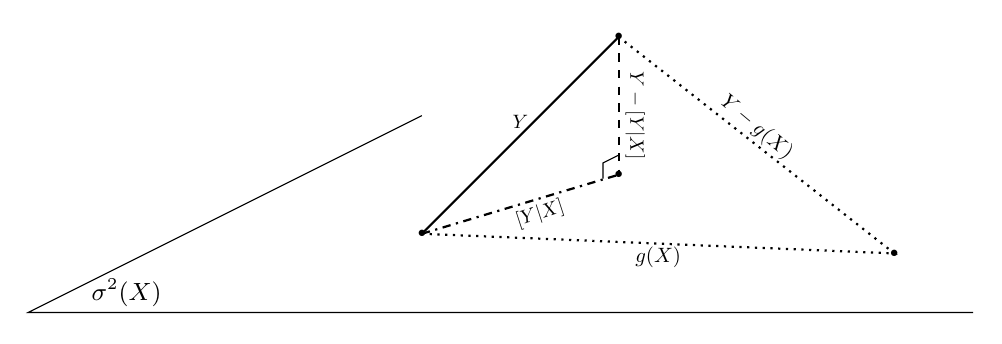
\begin{tikzpicture}%[scale=.9]
\shorthandoff{>}
%
\draw (5,2.5)--(0,0)--(12,0);
\draw (1.25,.25) node{\small $\sigma^2(X)$};
%
\draw[thick] (5,1) node[scale=.6]{$\bullet$} --(7.5,3.5) node[scale=.6]{$\bullet$};
\draw (6.25,2.25) node[above,scale=.7]{$Y$};
%
\draw[thick,dash dot] (5,1)--(7.5,1.75) node[scale=.6]{$\bullet$};
\draw (6.5,1.25) node[scale=.7]{\rotatebox{18}{$\Esp[Y|X]$}};
%
\draw[thick,dashed] (7.5,3.5)--(7.5,1.75);
\draw (7.5,2.5) node[right,scale=.7]{\rotatebox{-90}{$Y - \Esp[Y|X]$}};
\draw (7.3,1.7)--(7.3,1.9)--(7.5,2);
%
\draw[thick,dotted] (5,1)--(11,.75) node[scale=.6]{$\bullet$} --(7.5,3.5);
\draw (8,.7) node[scale=.75]{$g(X)$};
\draw (9.25,2.35) node[scale=.75]{\rotatebox{-40}{$Y-g(X)$}};
%
\end{tikzpicture}     \end{center}
  \leyenda{Ilustraci\'on del  teorema de  proyecci\'on ortogonal.  El  espacio \
    $\sigma^2(X)  = \{  g(X)  \: \forall  g  \: \mbox{medible  con}  \: g(X)  \:
    \mbox{de cuadrado integrable}\}$ \ es  representado por el plano y el vector
    representa $Y$. La linea punteada representa  la desviaci\'on \ $Y - g(X)$ \
    entre \ $Y$ \ y \ $g(X)$ \ dado \ $g(X) \in \sigma^2(X)$, siendo su cuadrado
    promedio  es m\'inimo  cuando (linea  con guiones)  \ $g(X)  =  \Esp[Y|X]$ \
    corresponde a la proyecci\'on ortogonal de \ $Y$ \ (linea mixta).}
\label{Fig:MP:TeoProyOrto}
\end{figure}
\end{proof}
%
A  veces,  este resultado  sirve  tambi\'en a  veces,  como  definici\'on de  la
esperanza condicional.